\chapter{Thực nghiệm của tác giả và phương pháp cải tiến của sinh viên}

Xem toàn bộ mã nguồn của sinh viên tại \url{https://github.com/hoangbaoan1901/tianen101}

\section{Thực nghiệm của tác giả}

\subsection{Tiền xử  lý dữ liệu}
Bộ dữ liệu đó được tác giả chia làm hai giai đoạn. Giai đoạn 1 với tập huấn luyện từ ngày 31 tháng 3 năm 2015 đến 31 tháng 3 năm 2018, tập test từ ngày 1 tháng 4 năm 2018 đến 30 tháng 9 năm 2018. Giai đoạn 2 với tập huấn luyện từ ngày 1 tháng 10 năm 2018 đến 30 tháng 9 năm 2021, tập test từ 1 tháng 10 năm 2021 đến 1 tháng 4 năm 2022.


\begin{figure}[h!]
    \centering
    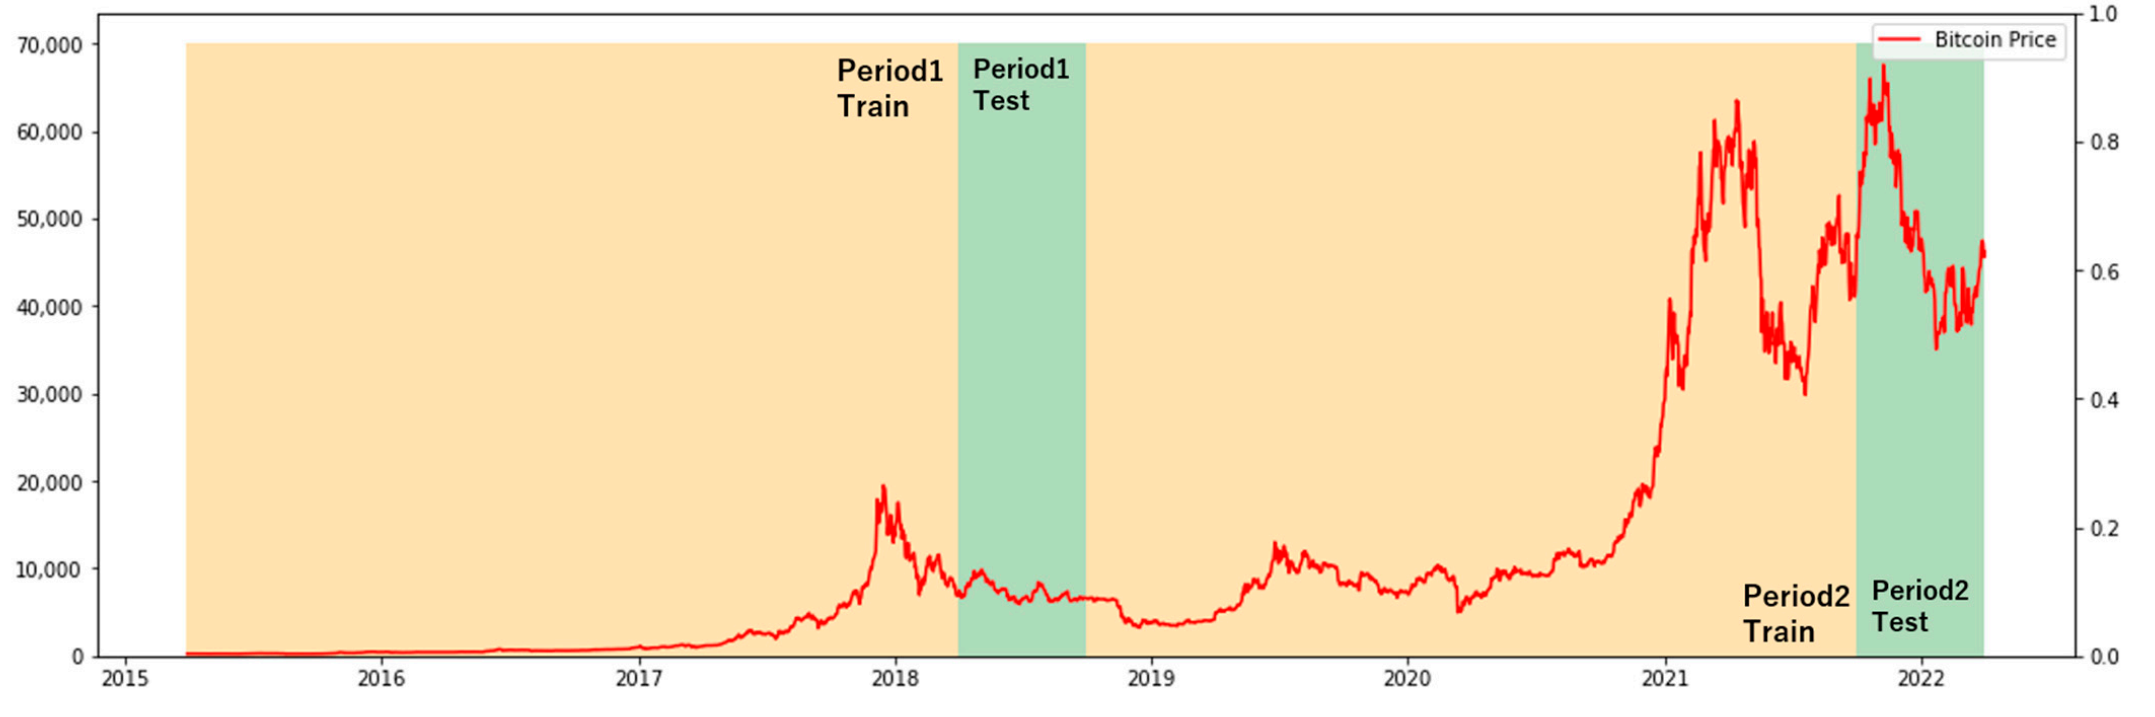
\includegraphics[width=\textwidth, keepaspectratio]{images/Chapter4/divine_dataset.png}
    \caption{Cách chia bộ dữ liệu của tác giả}
    \label{fig:divine_dataset}
\end{figure}


Vì hầu hết những dữ liệu bị thiếu là do những ngày nghỉ cuối tuần, ngày lễ, hoặc thảm họa, nên tác giả cũng đã đề xuất việc \textbf{forward-filling} cho bộ dữ liệu. Forward-filling là một kỹ thuật trong xử lý dữ liệu bị thiếu, nó sẽ điền giá trị bị thiếu bằng giá trị gần nhất mà không bị thiếu. Ở đây tức là giá trị của ngày hôm trước.

Với hầu hết các mô hình học sâu hiện tại, việc \textbf{chuẩn hóa dữ liệu} là điều cần thiết vì điều này sẽ khiến gradient hội hiệu quả hơn và giúp gradient hội tụ một cách cân đối. Ví dụ như việc các hàm kích hoạt như $ReLU$ và $sigmoid$ sẽ rất khó hội tụ khi giá trị âm quá lớn (với hàm $ReLU$) hoặc dương quá lớn thì sẽ khiến cho các hàm này rất khó hội tụ khi đã ở miền phẳng..

\subsection{Mô hình của tác giả}
Để tìm ra mô hình tốt nhất, tác giả đã sử dụng \textbf{GridSearchCV} từ gói phần mềm học máy \textbf{scikit-learn} để tìm ra bộ tham số tốt nhất cho cả hai mô hình tác giả đề xuất. 

Với mô hình Hồi quy Rừng ngẫu nhiên (Random Forest), tác giả sử dụng 500 cây quyết định với mỗi cây có độ sâu tối đa là 10. 

Sử dụng phương pháp tương tự, tác giả đề xuất một mô hình \textbf{LSTM} với 9 lớp (bao gồm một lớp output) như sau:

\begin{table}[hbpt]
    \centering
    \begin{tabular}{lll}
    \hline
    Layer & Layers & Parameters \\
    \hline
    Layer\_1 & LSTM\_1 & units: 128 \\
    & & Activation: ReLU \\
    Layer\_2 & Dropout\_1 & 0.2 \\
    Layer\_3 & LSTM\_2 & units: 128 \\
    & & Activation: ReLU \\
    Layer\_4 & Dropout\_2 & 0.3 \\
    Layer\_5 & LSTM\_3 & units: 256 \\
    & & Activation: ReLU \\
    Layer\_6 & Dropout\_3 & 0.4 \\
    Layer\_7 & LSTM\_4 & units: 256 \\
    & & Activation: ReLU \\
    Layer\_8 & Dropout\_4 & 0.5 \\
    Layer\_9 & Dense & units: 1 \\
    \hline
    \end{tabular}
    \caption{Mô hình LSTM được đề xuất}
    \label{tab:nn_architecture}
\end{table}

Activation function ở đây là hàm kích hoạt trạng thái (thông thường sẽ sử dụng hàm $tanh$), còn hàm kích hoạt hồi quy vẫn sẽ được sử dụng là hàm $sigmoid$.
Ngoài ra, một thông số nữa cũng khá quan trọng của các mô hình học sâu đó chính là epoch. Epoch là số lần mà toàn bộ dữ liệu được đưa qua mạng nơ-ron. Mỗi epoch sẽ được chia thành nhiều batch, và mỗi batch sẽ được đưa qua mạng nơ-ron. Ở giai đoạn 1, tác giả đã đề xuất cài đặt số epoch là 250, và giai đoạn 2, tác giả đã đề xuất cài đặt số epoch là 75.

\subsection{Các thang đo đánh giá mô hình}\label{sec: metrics}
Để đánh giá độ chính xác của một mô hình hồi quy, tác giả đã sử dụng các thang đo sau:
\begin{itemize}
    \item \textbf{Root Mean Squared Error (RMSE)}: RMSE là một thang đo đánh giá mức độ chênh lệch giữa giá trị dự đoán và giá trị thực tế. RMSE càng nhỏ thì mô hình càng tốt.
    \begin{equation}
        RMSE = \sqrt{\frac{1}{n}\sum_{i=1}^{n}(y_i - \hat{y}_i)^2}
    \end{equation}
    \item \textbf{Mean Absolute Percentage Error (MAPE)}: MAPE là một thang đo đánh giá mức độ chênh lệch giữa giá trị dự đoán và giá trị thực tế. MAPE càng nhỏ thì mô hình càng tốt.
    \begin{equation}
        MAPE = \frac{1}{n}\sum_{i=1}^{n}\left|\frac{y_i - \hat{y}_i}{y_i}\right|
    \end{equation}
    \item \textbf{Decision Accuracy (DA)}: DA là một thang đo đánh giá mức độ chính xác của mô hình. DA càng cao thì mô hình càng tốt. DA được tính bằng cách so sánh sự tăng hoặc giảm của giá trị dự đoán ngày hôm trước và ngày hôm sau. \textit{Nếu giá trị dự đoán và giá trị thực tế cùng tăng (hoặc cùng giảm) thì mô hình được tính là dự đoán đúng, ngược lại thì mô hình được tính là dự đoán sai.} Công thức tính DA như sau:
    \begin{equation}
        DA = (\frac{1}{n}\sum_{i=1}^{n}a(i)) * 100\%
    \end{equation}
\end{itemize}

Để so sánh kết quả giữa các mô hình, tác giả đã sử những giả thuyết kiểm định sau:
\begin{itemize}
   \item \textbf{Kiểm định Diebold-Mariano (DM)}: Nguyên lý của kiểm định DM có thể tóm tắt đơn giản như sau: cho hai tập chuỗi sai số dự đoán ${\{e'_t\}}^T_{t=1}$ và ${\{e_t\}}^T_{t=1}$, sau đó định nghĩa hàm mất mát $d_t = L(e_t) - L(e'_t)$, trong đó $L(e) = e^2$ là sai số bình phương trung bình (MSE) và $L(e) = |e|$ là sai số tuyệt đối trung bình (MAE).
   \begin{equation}
    DM_t = \frac{\overline{d_t}}{se(d_t)}
   \end{equation}
   \item \textbf{Kiểm định Clark-West}: Kiểm định Clark-West thêm vào thành phần $(e_t - e'_t)^2$ trong hàm mất mát của kiểm định Diebold-Mariano của MSE như sau: $f_t := (e_t)^2 - (e'_t)^2 + (e_t - e'_t)^2$, thành phần này cũng có phân phối tiệm cận $N(0,1)$, và cuối cùng thực hiện kiểm định giả thuyết một đuôi trên thống kê $f_t$
\end{itemize}

\subsection{Tổng quan quy trình thực nghiệm của tác giả}

\begin{figure}[h!]
    \centering
    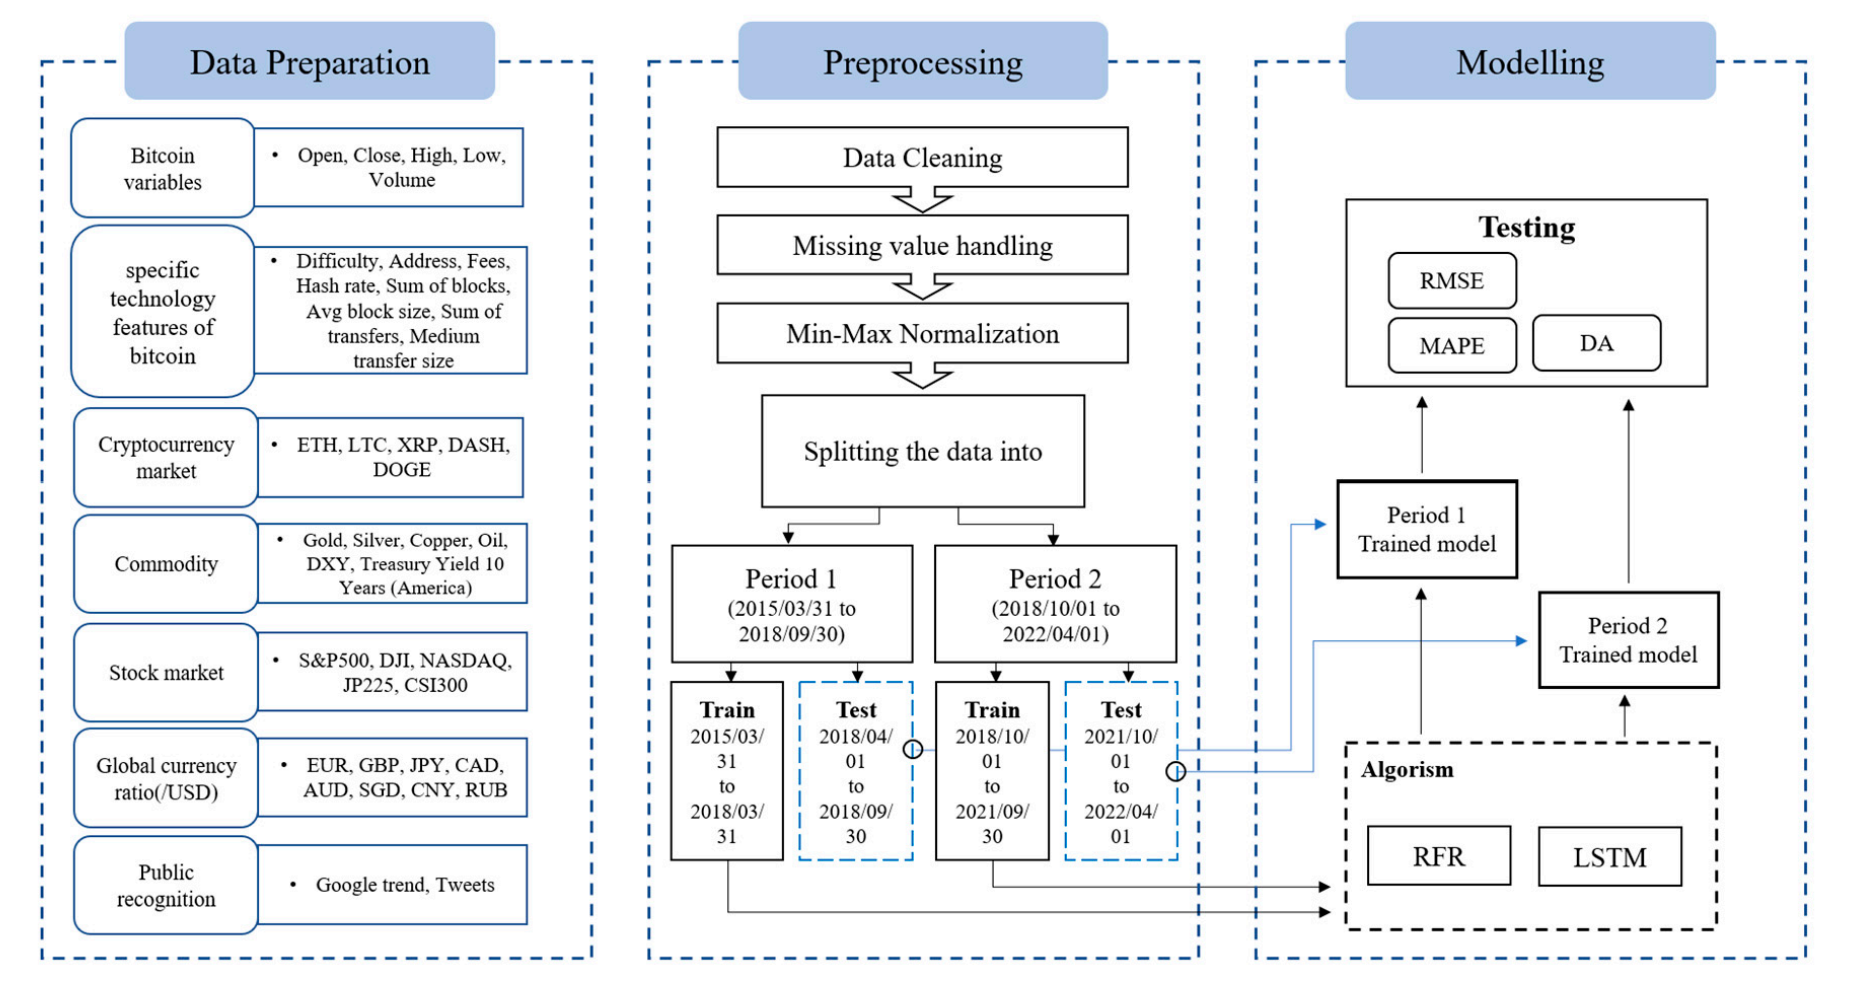
\includegraphics[width=\textwidth, keepaspectratio]{images/Chapter4/process.png}
    \caption{Tổng quan quy trình thực nghiệm tác giả}
    \label{fig:ori_process}
\end{figure}

\begin{table}[h]
    \centering
    \renewcommand{\arraystretch}{1} % Tăng khoảng cách giữa các dòng trong bảng
    \begin{tabular}{|p{7.5cm}|p{7.5cm}|}
        \hline
        \textbf{Ưu điểm} & \textbf{Nhược điểm} \\ \hline
        \begin{itemize}
            \item Forward-filling và chuẩn hóa giúp mô hình hội tụ tốt hơn.
            \item GridSearchCV tối ưu tham số mô hình.
            \item Random Forest với 500 cây giảm overfitting.
            \item LSTM phù hợp với dữ liệu chuỗi thời gian dài.
            \item Dropout giúp giảm overfitting trong LSTM.
            \item Số epoch được điều chỉnh hợp lý cho từng giai đoạn.
        \end{itemize} 
        & 
        \begin{itemize}
            \item Mô hình LSTM yêu cầu tài nguyên tính toán cao.
            \item LSTM có thể overfit nếu dữ liệu huấn luyện không đủ.
            \item Cần điều chỉnh tham số thủ công mất thời gian.
            \item Mô hình phức tạp, khó giải thích kết quả.
            \item Random Forest tính toán lâu với 500 cây.
            \item Cần phần cứng mạnh để huấn luyện nhanh.
        \end{itemize} \\ \hline
    \end{tabular}
    \caption{Ưu điểm và Nhược điểm của thực nghiệm tác giả}
    \label{tab:uudiem_hanche}
\end{table}

\section{Phương pháp cải tiến của sinh viên}
% Nói qua về cấu hình  (siêu tham số tối ưu)  + kết quả chạy (nhớ thêm ảnh kq)  của từng mô hình
% LUU Ý NHO NOI THEM VE CACH CHON va xu ly du lieu feature của từng model
\subsection{XGBoost (Extreme Gradient Boosting)}
\subsection{GRU}
\subsection{Stacking}

\section{So sánh và kết luận}
% Lap bảng so sánh -> Kết luận -> Giải thích tại sao nó tốt hơn ?
% CHÚ Ý so sánh với kết quả của tác giả TRONG BÀI BÁO nêu ra thôi